\documentclass[11pt,a4paper,titlepage]{article}
\usepackage[utf8]{inputenc}
\usepackage[english]{babel}
\usepackage[T1]{fontenc}

\RequirePackage[layout=inline]{fixme}

\usepackage{float}
\usepackage{graphicx}
\usepackage{setspace}
\usepackage{amsmath}
\usepackage{courier}
\usepackage{amsmath}
\usepackage{listings}
\usepackage{color}
\usepackage[toc, page]{appendix}

\usepackage[bottom]{footmisc}

\usepackage{changepage}

\definecolor{mygreen}{rgb}{0,0.6,0}
\definecolor{mygray}{rgb}{0.5,0.5,0.5}
\definecolor{mymauve}{rgb}{0.58,0,0.82}




\lstset{ %
	backgroundcolor=\color{white},   % choose the background color
	basicstyle=\scriptsize,        % size of fonts used for the code
	breaklines=true,                 % automatic line breaking only at whitespace
	captionpos=b,                    % sets the caption-position to bottom
	commentstyle=\color{mygreen},    % comment style
	escapeinside={\%*}{*)},          % if you want to add LaTeX within your code
	keywordstyle=\color{blue},       % keyword style
	stringstyle=\color{mymauve},     % string literal style
	numbers=left,
}

%\renewcommand{\thesubsection}{\thesection.\alph{subsection}}



\usepackage{booktabs}
\usepackage[backend=biber, bibencoding=utf8, style=ieee]{biblatex}

\addbibresource{../references.bib}
\usepackage[final,hidelinks]{hyperref} % must be last package loaded

\author{Ólafur Jón Thoroddsen}  % My name, for the titlepage
\title{\includegraphics{graphics/ru-logo}\\\vspace{10mm}
	Mechatronics II\\T-535-MECH \ \\Homework 5}  % The title, for the titlepage

\begin{document}
	\pagenumbering{arabic}
	\maketitle
	
	\tableofcontents
	\pagebreak
	
	\section{USART Communication}
	The USART peripheral on the ATmega328p enables serial communication with the processor. Figure~\ref{fig:overview} shows an overview of the MCU.
	
	\begin{figure}[h]
		\centering
		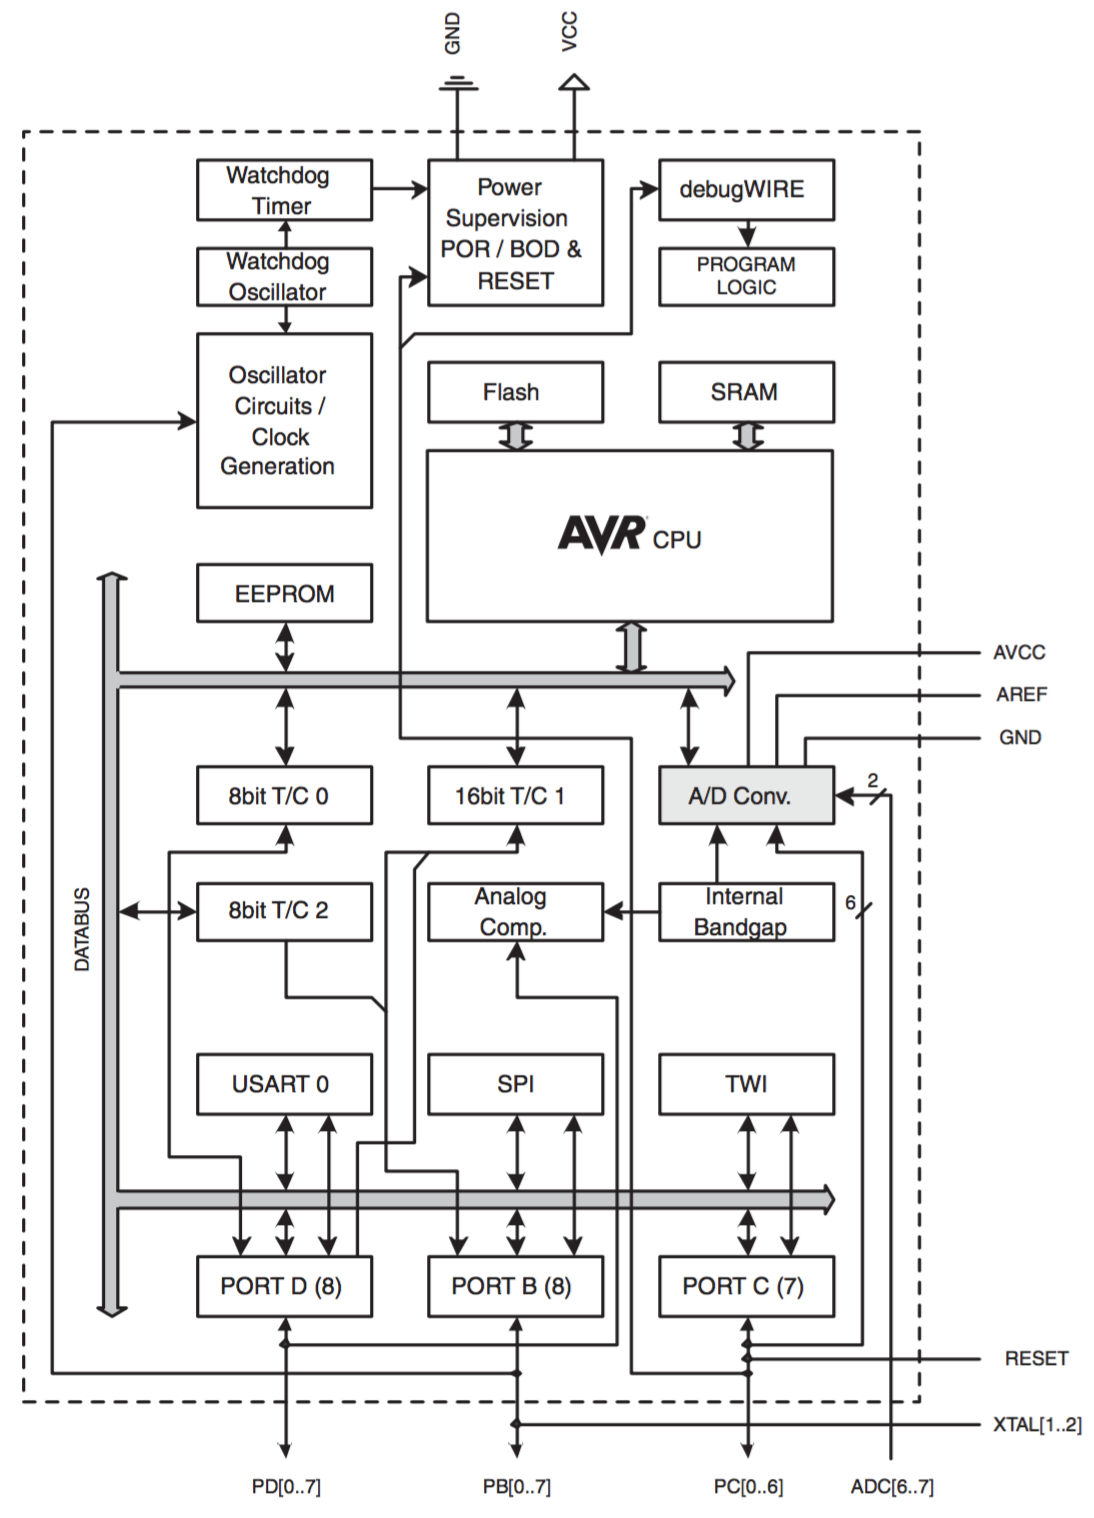
\includegraphics[width=0.5\textwidth]{graphics/overview}
		\caption{An overview of the ATmega328p MCU. The USART interface is shown in the lower left corner.}
		\label{fig:overview}
	\end{figure}
	
	\subsection{Initialization\label{sec:usartinit}}
	There are four registers that need to be set when initializing the USART. They are
	\begin{itemize}
		\item The USART Baud Rate Register High and Low (\verb|UBRR0H| and \verb|UBRR0L|): These two registers contain a value that is used along with counters to generate the desired baud rate. A special prescaled counter is decremented until it reaches the value stored in \verb|UBBR0H| and \verb|UBRR0L| at which time it sends out a pulse signal. For normal operation, the \verb|UBBR| value is calulated using eq.~\ref{eq:ubbr}
		\begin{equation}
			\verb|UBBR0| = \frac{f_{\text{OSC}}}{16\cdot\text{Baud Rate}} - 1
			\label{eq:ubbr}
		\end{equation}
		\lstinputlisting[language=c,firstline=11,lastline=14,frame=single,firstnumber=11]{../uart_echo/myUSART.c}
		For double speed or synchronous master modes, refer to pages 172-173 in~\cite{atmegadatasheet}
		
		\item The USART Control and Status Register B (\verb|UCSR0B|)  contains settings and flags that are used by the USART. 
		
		The \verb|RXEN0| and \verb|TXEN0| are the Receive and Transmit Enable bits and the \verb|RXCIE0| is the Receive Complete Interrupt Enable bit.
		 \lstinputlisting[language=c, frame=single,firstline=16,lastline=19,firstnumber=16]{../uart_echo/myUSART.c}
		 
		 \item The USART Control and Status Register C (\verb|UCSR0C|)  contains settings about the fame format of the sent and received data. For our purposes, we choose 8-bits of data with 2 stop bits.
		 \lstinputlisting[language=c,frame=single,firstline=21,lastline=23,firstnumber=21]{../uart_echo/myUSART.c}
	\end{itemize}
	
	\noindent Now that we have initialized communication over USART, we can start transmitting and receiving data.
	
	\subsection{Data reception}
	
	In this implementation, data reception is handled by an Interrupt Service Routine each time the \verb|RXC0| flag is set in the \verb|UCSR0A| register.
	
	Each time data is written to the USART from a terminal program, the \verb|RXC0| flag is set and the ISR is executed. There the data from the USART I/O Data Register (\verb|UDR0|) is written to the buffer \verb|rxBuffer|. The \verb|dataReceived| variable is a flag to indicate to the main program that new data is available in the buffer. It has to be manually set to logical 0 when the data has been read from the buffer.
	
	\lstinputlisting[language=c,frame=single,firstline=47,lastline=52,firstnumber=47]{../uart_echo/myUSART.c}

	\subsection{Data transmission}
	
	Data is transmitted from the ATmega328p by a polling function. When called, it waits until the USART I/O Data Register (\verb|UDR0|) is empty, indicated by the \verb|UDRE0| flag in \verb|UCSR0A| and then writes data to \verb|UDR0| .
	
	\lstinputlisting[language=c,firstline=27,lastline=34,frame=single,firstnumber=27]{../uart_echo/myUSART.c}

	\subsection{Echo}
	
	To test the USART implementation, a simple echo program was written.
	The value of the \verb|UBRR0| register is calculated in the beginning of the program and stored in the \verb|MYBRR| constant.
	After initialization, the global interrupt flag is enabled in the \verb|SREG|. Then the loop runs continuously until the \verb|USART_RX| interrupt is executed, where the \verb|dataReceived| flag is set to logical 1. Then the data from the \verb|rxBuffer| is written to the transmitter, echoing back the received data. \verb|dataRecevied| is set to logical 0 to "close the connection" and the \verb|rxBuffer| is cleared for future data receptions (This might be redundant but I feel like it's not a good idea to leave data in a buffer). An example of how the program works is shown in figure~\ref{fig:message}.
	
	\lstinputlisting[language=c,frame=single,firstline=8,lastline=27,firstnumber=8]{../uart_echo/main.c}
	
	\begin{figure}[h]
		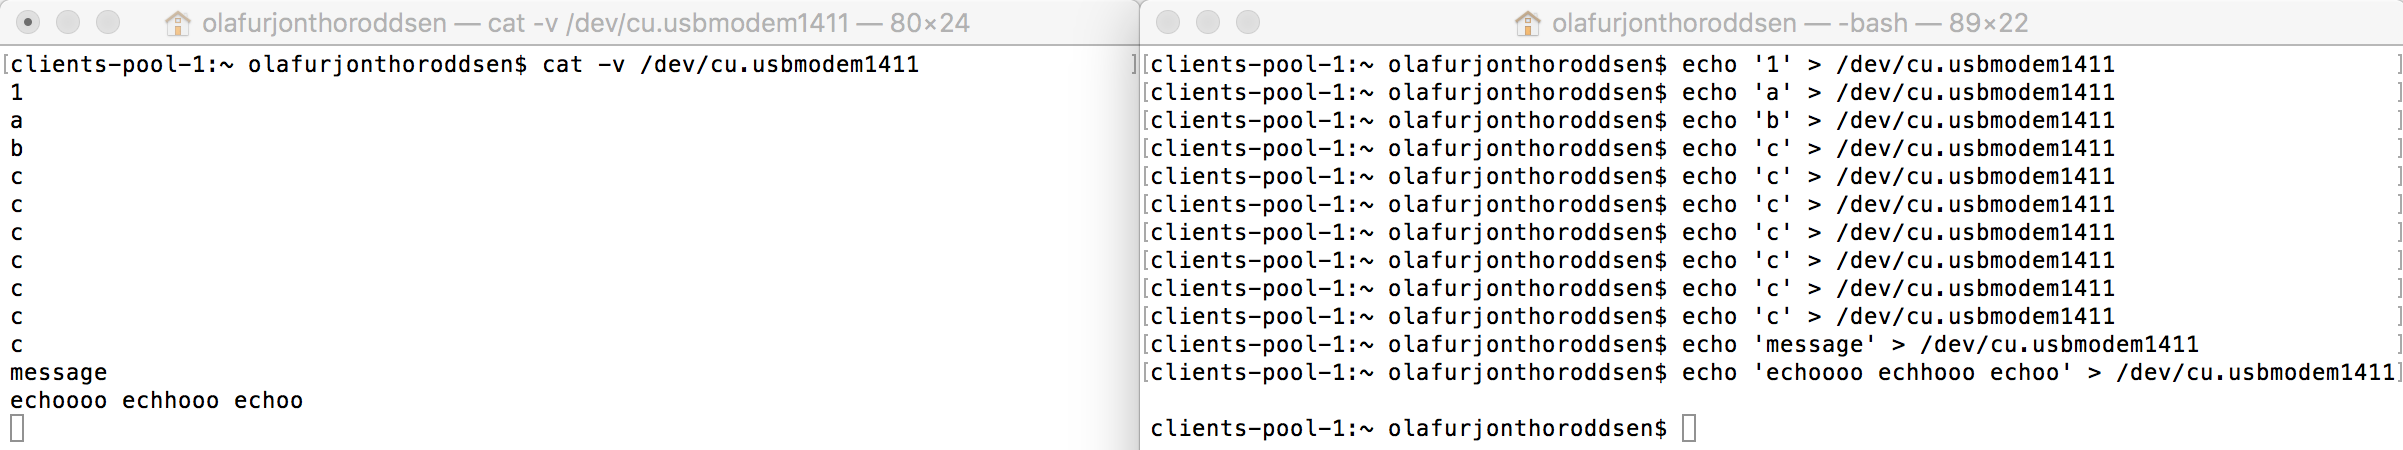
\includegraphics[width=\textwidth]{graphics/message}
		\caption{Demonstration of the Echo program in a terminal window. The left window is listening to the port /dev/cu.usbmodem1411 and the right window is writing data to it.}
		\label{fig:message}
	\end{figure}
	
	\pagebreak
	\section{USART controlled PWM signal\label{sec:usartpwm}}
	
	The USART is very flexible and can be used for general communication from a device, such as a computer, to the MCU. Because of that, we can define control signals in our program and use them to set values to variables or even manipulate registers.
	In this exercise, I used USART communications to change the value of the Output Compare Register B (\verb|OCR0B|) to vary the Duty Cycle of a PWM signal.
	
	The program consists of three libraries, a clock library for setting up the timer/counter appropriately, an LED library for turning a diode on and off, and the USART communications library also used in the previous section.
	The entire code for all libraries and the main program can be seen in the appendix.
	
	\subsection{Clock initialization \label{sec:clock}}
	To initialize the clock, there are five registers that we want to manipulate.
	\begin{itemize}
		\item The Timer/Counter Control Register B (\verb|TCCR0B|) is used to select the clock prescaling. I chose 1/64th prescaling.
		\lstinputlisting[language=c,frame=single,firstline=12,lastline=14,firstnumber=12]{../uart_pwm_led/clockFuncs.c}
		
		\item The Timer/Counter Register (\verb|TCNT0|) is the actual counter that gets incremented every 64 clock cycles. In the initialization, we ensure it will start at zero.
		\lstinputlisting[language=c,frame=single,firstline=15,lastline=16,firstnumber=15]{../uart_pwm_led/clockFuncs.c}
		
		\item The Timer/Counter Interrupt Mask Register (\verb|TIMSK0|) is used to enable interrupts on Output Compare and Timer Overflow.
		\lstinputlisting[language=c,frame=single,firstline=17,lastline=18,firstnumber=17]{../uart_pwm_led/clockFuncs.c}
		
		\item The Timer/Counter 0 Interrupt Flag Register (\verb|TIFR0|) contains the flags for the Compare Match and Timer Overflow interrupts.
		\lstinputlisting[language=c,frame=single,firstline=19,lastline=20,firstnumber=19]{../uart_pwm_led/clockFuncs.c}
	\end{itemize}
	
	\subsection{Main program}
	The main program begins by enabling global interrupts and initializing the clock using the function described in section~\ref{sec:clock}. Then the USART is initialized using the function in section~\ref{sec:usartinit} and an LED is initialized on pin 12 on the Arduino board. Then, to have the LED turned on when the board starts up, we call the \verb|setLedPWM| function with some value between 0 and 100.
	
	\lstinputlisting[language=c,frame=single,firstline=34,lastline=75, firstnumber=33]{../uart_pwm_led/main.c}
	
	\subsubsection{setLedPWM}
	This function is designed to update the Output Compare Register B. The input to the function is a value between 0 and 100, 0 means that the duty cycle of the PWM signal should be 0\% of the frequency and 100 means that it should be 100\% of the frequency. The input is sanitized such that if the user inputs an illegal value ( intensity $\notin$ [0,100]~), it will be forced to either 0 or 100 depending on the input.
	
	\lstinputlisting[language=c,frame=single,firstline=28,lastline=31,firstnumber=28]{../uart_pwm_led/main.c}
	
	\subsubsection{Interrupt Service Routines}
	
	To create the PWM signal, two ISRs are used. The Output Compare ISR and the Timer Overflow ISR. They are responsible for turning the LED on and off and by changing the value of \verb|OCR0B|, we can generate a PWM signal with a variable duty cycle.
	
	\lstinputlisting[language=c,frame=single,firstline=20,lastline=22,firstnumber=20]{../uart_pwm_led/main.c}
	\lstinputlisting[language=c,frame=single,firstline=24,lastline=26,firstnumber=22]{../uart_pwm_led/main.c}
	
	\subsection{Assembly output}
	Looking at the assembly output of a compiled program can give clues about how to optimize the program.
	\subsubsection{Compare Match Interrupt \& Led\_on()}
	The ISR assembly code for the Compare Match interrupt is shown here below.  There are a lot of registers pushed to the stack in this ISR because of previous variables used in the program. Counting the clock cycles yields 79~cs for the ISR and if we include the cycles in the Led\_on() function that is called, the total number of cycles is 108. 
	\lstinputlisting[frame=single,firstline=226,lastline=269,firstnumber=226]{../uart_pwm_led/Debug/uart_pwm_led.lss}
	\lstinputlisting[frame=single,firstline=112,lastline=130,firstnumber=112]{../uart_pwm_led/Debug/uart_pwm_led.lss}
	
	\subsubsection{Timer Overflow Interrupt \& Led\_off()}
	The ISR assembly code for the Timer Overflow interrupt is shown here below. Again as with the other routine, there are a lot of registers pushed to the stack that then need to be popped off again. Summing up the clock cycles for the ISR and the Led\_off() function yields 110 cycles. This might be optimized by reducing the number of variables if possible.
	
	\lstinputlisting[frame=single,firstline=273,lastline=316,firstnumber=273]{../uart_pwm_led/Debug/uart_pwm_led.lss}
	\lstinputlisting[frame=single,firstline=134,lastline=152,firstnumber=134]{../uart_pwm_led/Debug/uart_pwm_led.lss}	
	
	\pagebreak
	\section{Progress with my project}
	
	\subsection{Last week}
	This week I worked hard on the communications module using USART which I intend to use extensively in my project for debugging. I also worked hard on learning all the nuts and bolts of the timers on the ATmega and created my own PWM module as described in section~\ref{sec:usartpwm}. This module could possibly be improved by the build in PWM functionalities in the ATmega but that is a project for next week to find out. I obtained some materials to build with. I have some thin wood I intend to use for the chassis of the robot and I have acquired two small geared DC motors and brackets to keep them in place as well as two lithium polymer batteries. I intend to test the power consumption of the equipment before connecting batteries to it to make sure everything will be (theoretically) all right. 
	
	
	\subsection{Next week}
	
	\begin{table}[h]
		\centering
		\begin{tabular}{llc}
			\toprule
			Task no.	&	Task	&	ETC\footnotemark\\
			\midrule
			1	&	\begin{tabular}{@{}l@{}}Write an interface module to\\talk with the IMU sensor\end{tabular} &	10 hours \\	
			\midrule	
			2	&	\begin{tabular}{@{}l@{}}Find out if the PWM\\ functionalities in ATmega are\\worth replacing my own with.\end{tabular}	&	2 hours\\
			\midrule
			3	&	\begin{tabular}{@{}l@{}}If worth pursuing further, write a \\PWM module using the ATmega\\built in functionalities\end{tabular}	&	10 hours\\
			\midrule
			4	&	\begin{tabular}{@{}l@{}}Have a mockup of the robot ready by the\\end of the week. A quick prototype to\\get a better feel of the scale.\end{tabular}	&	10 hours\\
			\bottomrule
		\end{tabular}
		\label{tab:nextweek}
	\end{table}
	
	
	\footnotetext{Estimated Time to Complete}
	\pagebreak
	\subsection{Long term plan}
	
	\begin{table}[h]
		\centering
		\hspace*{-2cm}
		\begin{tabular}{lccc}
			\toprule
			Week	&	Software design	&	Mechanical design	&	Testing\\
			\midrule
			6	&	IMU \& PWM	&	1st prototype	&	Serial communication\\
			\midrule
			7	&	PID motor control	&	Robot chassis	&	IMU \& PWM\\
			\midrule
			8	&	Rethink IMU \& PWM	&	\begin{tabular}{@{}l@{}}Power circuitry\\2nd prototype\end{tabular}	&	\begin{tabular}{@{}l@{}}Estimate power consumption\\PID motor control\end{tabular}\\
			\midrule
			9	&	Rethink PID control	&	3D drawing of the robot	&	Power consumption	\\
			\midrule
			10	&	\begin{tabular}{@{}l@{}}Integrate IMU, PID\\ and PWM modules\end{tabular}	&	Altium schematics of electronics	&	Integration\\
			\midrule
			11	&	Integration	&	Integration	&	Integration	\\
			\midrule
			12	&	Everything	&	Report layout design	&	Integration	\\
			\bottomrule
		\end{tabular}
		\label{tab:longterm}
		\hspace*{-2cm}
	\end{table}
	
	
\pagebreak
\section*{Appendices}
\appendix
\section{main.c}
\lstinputlisting[language=c,frame=single]{../uart_pwm_led/main.c}
\section{main.c Assembly}
\lstinputlisting[frame=single,firstline=368,lastline=471,firstnumber=368]{../uart_pwm_led/Debug/uart_pwm_led.lss}
\section{Led.c}
\lstinputlisting[language=c,frame=single]{../uart_pwm_led/Led.c}
\section{myUSART.c}
\lstinputlisting[language=c,frame=single]{../uart_pwm_led/myUSART.c}
\section{clockFuncs.c}
\lstinputlisting[language=c,frame=single]{../uart_pwm_led/clockFuncs.c}

\pagebreak
\printbibliography

\end{document}